\section{直言命题的标准化}

\begin{quotation}
本节介绍将日常语言中的非标准直言命题翻译为标准形式的九种方法。这些方法帮助我们将各种复杂的语言表达转换为可以用标准三段论规则和文恩图检验的形式,从而正确评估其有效性。
\end{quotation}

如 7.1 节所述,日常语言中三段论论证的形式可能偏离标准形式,不仅可能出现含有三个以上词项的情况(如 7.2 节讨论的那样),还可能有

这样的情况,即构成命题不都是标准的直言命题。显然,A、E、I、O命题有些生硬,而日常生活中许多三段论都是由非标准的命题组成的。要把这些论证化归为标准形式,就要把构成命题都翻译为标准形式。但日常语言内容丰富、形式多样,根本无法找出一套完善的翻译规则。在各种情形中,最关键的是理解已知的非标准命题的含义,这样才能在翻译时不丢失,也不改变原意。

尽管没有完善的规则,我们仍然可以介绍一些方便的方法,它们在处理某些特殊命题时常常十分有用。这些方法——本节介绍九种方法——只能被看做一种指针而不是规则,也就是说,它们是处理某些特定种类的非标准命题的技巧。

1.单称命题。有些命题肯定或否定的是一个特定的个体或对象属于某个类,例如"苏格拉底是哲学家"、"这张桌子不是古董"等。这样的命题叫做\textbf{单称命题}。它们肯定或否定的不是一个类与另一个类的包含关系 (像标准式直言命题那样),但我们可以把单称命题解释为处理类与类间关系的命题。可以按如下方式做到这一点:

每一个个体对象都对应着一个\textbf{单元类}(由一个元素组成的类),其中只有一个对象。这样,断定一个对象 $s$ 属于类 $P$ ,在逻辑上等价于断定了只含有一个元素的单元集 $S$ 完全包含于类 $P$ 之中。而断定一个对象 $s$ 不属于类 $P$ ,在逻辑上等价于断定只含有一个元素的单元类 $S$ 完全排斥在类 $P$之外。通常将这种解释看做自然而然的,无须调整记法。据此,我们就可以将任何一个单称肯定命题"$s$ 是 $P$"看做逻辑上等价的 A 命题"所有 $S$是 $P$"。同样,可以简单地将单称否定命题"$s$ 不是 $P$"看做逻辑上等价的 E 命题"没有 $S$ 是 $P$"——S 指称的都是只有一个对象 $s$ 的单元类。因此,不需要对单称命题进行明确的翻译,一般把它们分别归到 $\mathrm{A} 、 \mathrm{E}$ 命题当中。康德说过"在三段论中判断之使用,逻辑学者把单称判断类如全称判断处理,是很恰当的"${ }^{[1]}$ 。

然而,情况并不那么简单。特称命题有存在含义,而全称命题没有。在布尔解释下(如5.6节说明),如果机械地把单称命题当做三段论推理的 A、E 命题;再用文恩图或三段论规则来检验其有效性,就会出现严重的困难。

很明显,在某些情况中,可以把含单称命题的有效的两前提论证转化为有效的三段论。例如:

$$
\begin{array}{ll}
\text { 所有 } H \text { 是 } M, & \text { 可以变为三段论的 Barba- } \\
\frac{s \text { 是 } H,}{\therefore s \text { 是 } M_{0}} & \text { ra, 即 AAA-1 式, 很明显 } \\
\text { 是有效的 } &
\end{array}
$$

$$
\begin{aligned}
& \text { 所有 } H \text { 是 } M, \\
& \text { 所有 } S \text { 是 } H, \\
& \therefore \text { 所有 } S \text { 是 } M \text { 。 }
\end{aligned}
$$

但在另外的某些情形下,把含单称命题的有效的两前提论证转化为三段论,却是明显无效的。例如:

$$
\begin{array}{ll}
s \text { 是 } M, & \text { 得到的直言三段论是无效 } \\
\frac{s \text { 是 } H,}{\therefore \text { 有 } H \text { 是 } M_{0}} & \text { 的 AAI-3 式 }
\end{array}
$$

后者违反了规则 6 ,犯了存在谬误。\\
再者,如果把单称命题转化为特称命题,也会有同样的困难。有些情况下转化是有效的,例如:

\begin{center}
\begin{tabular}{lll}
所有 $H$ 是 $M$, & 可以变为三段论的 Darii, & 所有 $H$ 是 $M$, \\
$\frac{s \text { 是 } H,}{\therefore s \text { 是 } M \text { 。 }}$ & 即 AII-1 式,很明显是有效的 & 有 $S$ 是 $H$, \\
$\therefore$ 有 $S$ 是 $M$ 。 &  &  \\
\end{tabular}
\end{center}

但在另一些情况中,这种翻译却会得出明显无效的直言三段论。例如:

\begin{center}
\begin{tabular}{lll}
$s$ 是 $M$, & 得到的直言三段论是无效的 & 有 $S$ 是 $M$, \\
$\frac{s \text { 是 } H,}{\therefore}$ 有 $H$ 是 $M$ 。 & 有 $S$ 是 $H$, &  \\
$\therefore$ & 有 $H$ 是 $M$ 。 &  \\
\end{tabular}
\end{center}

后者违反了规则 2 ,犯了中项不周延谬误。\\
问题来自如下事实:单称命题要比任何一个标准式命题负载更多信息。如果把"$s$ 是 $P$"当做"所有 $S$ 是 $P$",那么,就丢掉了单称命题的存在含义,实际上这里 $S$ 非空。而如果把"$s$ 是 $P$"当做"有 $S$ 是 $P$",又漏掉了单称命题的全称性,即主项周延,它说的是全部 $S$ 是 $P$ 。

解决此问题的办法,就是把单称命题分析为两个直言命题的合取,即

一个单称肯定命题等价于相互关联着的 A、I 命题的合取。这样"$s$ 是 $P$"就等价于"所有 $S$ 是 $P$"合取"有 $S$ 是 $P$",单称否定命题则等价于"没有 $S$ 是 $P$"合取"有 $S$ 不是 $P$"。图7—1就是单称命题的肯定式和否定式的文恩图。在用三段论规则评估这种推理时,必须考虑它提供的所有信息,既考虑周延性也考虑存在含义。\\
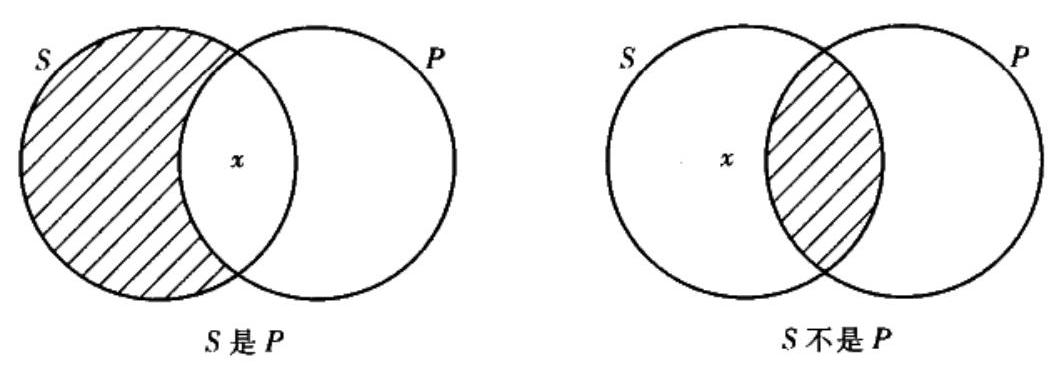
\includegraphics[width=\textwidth]{images/2025_05_15_6a28331d5e7c993ad07ag-310.jpg}

图7—1\\
对于含有单称命题的三段论,引用文恩图或规则检验其有效性时,只要我们记住其中有存在含义,就可以直接把它们看做全称(A 或 E )命题。

2.谓项为形容词或形容词短语,而非名词或类词项的直言命题。例如"有花是美的"、"没有战船是可调用的"都是直言命题,但"美的"和 "可调用的"表示的只是属性而不是类,所以它们的形式不标准,必须转化为标准形式。不过,每个属性都可以确定一个类,即具有这种属性的事物组成的类,所以对于每个这样的命题,都有一个相应的标准式直言命题。两个例句分别对应的是:I命题"有花是美的事物"和 E 命题"没有战船是可调用的事物"。如果一个直言命题的形式是标准的,只有谓项为形容词或形容词短语时,就把形容词或短语替换为这样一个词项,它指称由所有具有形容词表示之属性的事物所组成的类。

3.主要动词不是标准的联项"是"或"不是"的直言命题。常见的例子有"所有人都寻求赞誉"、"有人饮用希腊酒"。通常,转化的方法是把主项和量项之外的所有成分看做类的定义特征。先把能被替换的成分换成这样的词项,它们指称由类定义特征所确定的类,再改用标准的联项把它们同主项联结起来。这样上面两个例子就成了:"所有人是赞誉的寻求者"、"有人是希腊酒的饮用者"。

4.标准形式的各成分都出现,却没有按标准顺序排列的陈述句。"赛马全是良种马"和"结果好的事总是好事"就是这样的例子。在这种情形

下,首先要找出哪个是主项,然后再重新把各个成分排列一下,使之成为标准式直言命题。这种翻译通常都很直接。十分清楚,上述两个例句可翻译为"所有赛马是良种马"和"所有结果好的事是好事"。

5.量词不是"所有"、"没有"和"有"这些标准语词的直言命题。以 "每一"、"任何"等开头的陈述句很好转化。"每一只狗都有其得意之时"、 "任何贡献都会得到赞赏"可分别转化为"所有狗是有其得意之时的动物"和"所有贡献是会得到赞赏的事情"。"每一事物"、"任何东西"类似于 "每一"、"任一"。与此同一系列但限于人类的是"每人"、"任何人"、"无论谁"、"不管是谁"、"那些……的人"以及"每个......的人"等等。以上各表达式都不会带来什么麻烦。

语法冠词"a"和"an"("一个"等)也可用于指代量词,必须依据当时的语境,确定它们的意思是"所有"还是"有"。例如,"A bat is a mammal"(一只蝙蝠是一个哺乳动物)与"An elephant is a pachyderm" (一头大象是一个厚皮动物)可以合理地解释为"所有蝙蝠都是哺乳动物"与"所有大象都是厚皮动物"。但"A bat flew in the window"(一只蝙蝠飞进窗户)和"An elephant escaped"(一头大象逃跑了)显然指的是 "有蝙蝠是飞进窗户的动物"和"有大象是逃跑的动物"。

冠词"the"("这"、"这些"等)既可以用于指称一个特定的个体,也可以指称一个类的全部元素,有可能引起混淆。例如"The whale is a mammal"(鲸是哺乳动物)这句话,在一般情况下都会被理解为"所有鲸都是哺乳动物",而单称命题"The first president was a military hero" (第一任总统是军旅英雄)可以说是标准形式的 A 命题(一个有存在含义的单称命题),其道理本节前面已经讨论过了。 ${ }^{[2]}$

尽管以"每一"和"任一"开头的肯定句都可以译为"所有 $S$ 是 $P$",但对于以"not every"(并非每一个)和"not any"(并非任一)开头的否定句,却有很大区别。它们的译法不那么明确,需要更加小心。比如, "Not every $S$ is $P$"意思是有 $S$ 不是 $P$ ,而"Not any $S$ is $P$"意思是没有 $S$ 是 $P$ 。

6.排斥命题(exclusive propositions)。含有"只"(only)、"只有"(none but)的直言命题通常叫做\textbf{排斥命题},因为一般说来,它们断言的是谓项排他性地适用于主项。例如"只有公民能成为选民"、"只有勇敢者是值得公平对待的",第一句转化为标准形式是"所有能成为选民的是公

民",第二句转化为"所有值得公平对待的人是勇敢者"。以"只"、"只有"开头的命题一般可以按以下途径转化为 A 命题:将主、谓项互换位置,把"只有"换为"所有"。因此"只有 $S$ 是 $P$"和"只有 $S$'s 是 $P$'$s$"通常被理解为"所有 $P$ 是 $S$"。

但是,在某些语境中,"只"、"只有"被用于表达某种更多的含义。 "只有 $S$ 是 $P$"和"只有 $S$'s 是 $P$'$s$"表明的可能是"所有 $S$ 是 $P$"或者 "有 $S$ 是 $P$"。但这种情况并不常见。这个时候就需要语境的辅助了。如果没有附加信息,前面的翻译就是适当的。

7.不含量词的直言命题。例如"狗是肉食动物"、"孩子在场"。欠缺量词,句子的含义就不十分明确。只有考察它们所处的语境才能确定其含义,一般来说,考察之后就能把疑义清理掉。第一个例句"狗是肉食动物"很可能述及了所有的狗,可以转化为"所有狗都是肉食动物"。而第二个例句一般只述及某些孩子,转化为标准形式为"有孩子是在场的人"。

8.完全不像标准式直言命题但也可以有标准式翻版的命题。例如 "不是所有孩子都相信圣诞老人"、"有白色的大象"、"没有粉色的大象"以及"没有既圆又方的东西"。反思这些命题就会发现,它们在逻辑上等价于(因而可翻译为)下面的标准式命题:"有孩子不是相信圣诞老人的人"、"有大象是白色的事物"、"没有大象是粉色的事物"和"没有圆的东西是方的"。

9.除外命题(exceptive propositions)。还有一些这样的例子:"除了雇员(all except)都是合格的"、"雇员之外的人(all but)都是合格的"与"只有(alone)雇员不是合格的"。要把这样的\textbf{除外命题}翻译为标准形式,情况就会复杂一些,因为这种命题(与单称命题很类似)做出了两个而不是一个方面的断定。所给例子断言的不仅是所有非雇员是合格的,还断定了(在通常的语境中)没有雇员是合格的。如果把"雇员"记为 $S$ 、 "合格的人"记为 $P$ ,那么,这两个命题可以写成"所有非 $S$ 是 $P$"和 "没有 $S$ 是 $P$"。这两个命题是独立的,但联合起来就断定了 $S$ 和 $P$ 互为补类。

每个除外命题都是复合句,因此,不能转化为单一的标准式直言命题。确切地说,每一个除外命题应当翻译为一个合取式,即两个标准式直言命题的合取式。所以,上面关于合格性的三个例句都可以翻译为"所有非雇员是合格者,并且没有雇员是合格者"。

应该注意到,有些论证的有效性离不开数字或类数字(quasi-numeri- cal),但数字无法译为标准形式。这些推理本身就是非三段论的(asyllo- gistic)。因此,对它们进行分析就需要一种比直言三段论复杂一些的理论。当然,有些含有类数字量词的推理也可以用三段论分析。"几乎所有"、"并非全部"、"除少数几个之外都"、"几乎每个人"等就是这样的词。如果一个命题含有看起来像量词的词项,那么就可以处理为刚刚讲过的除外命题。下面几个除外命题都含有类数字:"几乎所有学生都参加了舞会"、"并非所有学生都参加了舞会"、"除少数几个之外,学生们都参加了舞会"和"只有一些学生参加了舞会",它们都肯定了有些学生参加了舞会,同时又否定了所有学生都参加了舞会。从三段论推论的观点看,它们给出的类数字信息并不相干,转化之后都是"有学生是参加了舞会的人,并且有学生不是参加了舞会的人"。

由于除外命题不是直言命题,而是合取式,含有这些命题的论证并不是我们所说的三段论论证。但是,对它们进行三段论分析和评估也未尝不可。含有除外命题的论证,要依据该命题所处的位置来进行检验。如果它是前提,那么就要分两次进行检验。举例来说,看下面这个论证:

\begin{quote}
每个看过比赛的人都参加了舞会,

不是全体学生都参加了舞会,

所以,有学生没有看过比赛。
\end{quote}

其中,第一个前提以及结论都是直言命题,很容易译为标准形式。但第二个前提是一个除外命题,不是简单句而是复合句。要检查前提是否蕴涵结论,首先要检验由论证的第一个前提、第二个前提的前一半以及结论组成的三段论。我们有:

\begin{quote}
所有看过比赛的人都是参加了舞会的人,

有学生是参加了舞会的人,

所以,有学生不是看过比赛的人。
\end{quote}

这个标准式的直言三段论是 AIO-2,违反了规则 2,犯了中项不周延的谬

误。但不能由此就得出结论说原来的论证是无效的,因为受检验的三段论只包含它的一部分前提。现在再来检验由第一个前提、第二个前提的后一半以及结论组成的三段论。译为标准形式后,得到一个非常不同的三段论:

所有看过比赛的人都是参加了舞会的人,\\
有学生不是参加了舞会的人,\\
所以,有学生不是看过比赛的人。

这是一个标准的 Baroko,即三段论的 AOO-2。很容易看出它是有效的。原来的三段论与这个有效式的结论相同,并且前者的前提包含着后者的前提,所以原来的论证也是有效的。因此,如果一个论证中有一个前提是除外命题,那么,对其有效性的检验要分为两次,即分别对两个不同的标准式直言三段论进行检验。

如果前提都是直言命题,但结论是除外命题,那么我们就可断言它是无效的。尽管两个直言命题可以蕴涵其中一个,即蕴涵结论复合句的一半,但不可能同时蕴涵两个。最后,如果两个前提和结论都是除外命题的话,那么,由原来论证所能建构的任何一个可能的三段论都要接受检验,才能确定其有效性。以上解释已足够处理这种情况了。

学会将多种非标准命题翻译为标准形式的技巧是很重要的,因为我们已经掌握的检验方法——文恩图解和三段论规则——只能直接用于标准式直言三段论。

\begin{center}
\fbox{\parbox{0.95\textwidth}{
\textbf{本节要点}
\begin{itemize}
\item 将非标准直言命题转换为标准形式的九种方法:
  \begin{itemize}
  \item \textbf{单称命题}:可将"苏格拉底是哲学家"视作"所有S是P",但须注意其包含存在含义
  \item \textbf{谓项为形容词的命题}:将形容词改写为对应的名词类型,如"美的"改为"美的事物"
  \item \textbf{非标准联项的命题}:将非"是/不是"动词改写为标准联项结构
  \item \textbf{顺序不标准的命题}:重新排列成分以符合标准顺序
  \item \textbf{量词不标准的命题}:将各类非标准量词("每一"、"任何"等)转换为标准量词
  \item \textbf{排斥命题}:"只有S是P"转换为"所有P是S"
  \item \textbf{不含量词的命题}:根据语境补充适当量词
  \item \textbf{非标准形式但可翻译的命题}:寻找逻辑等价的标准形式表达
  \item \textbf{除外命题}:翻译为两个标准式命题的合取
  \end{itemize}
\item 转换的核心原则是保持原命题的逻辑含义不变
\item 对含有除外命题的论证,需要分别对其组成部分进行有效性检验
\end{itemize}
}}
\end{center} 